\documentclass[tikz,border=3.14mm]{standalone}
\usetikzlibrary{matrix,quotes,positioning}

\begin{document}
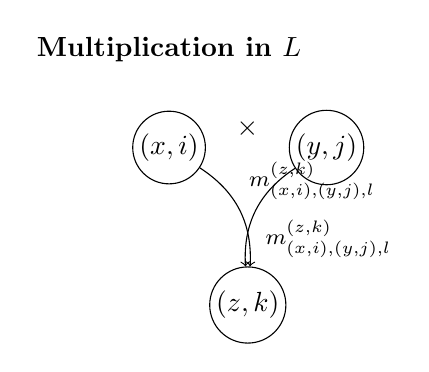
\begin{tikzpicture}[
    node distance=2cm,
    every edge quotes/.append style={auto,font=\footnotesize},
    basis/.style={draw,circle,inner sep=1pt}
]
    % Basis elements as nodes
    \node[basis] (x) at (0,0) {$(x,i)$};
    \node[basis] (y) at (2,0) {$(y,j)$};
    \node[basis] (z) at (1,-2) {$(z,k)$};
    
    % Arrows representing multiplication with coefficients
    \draw[->] (x) edge[bend left,"$m_{(x,i),(y,j),l}^{(z,k)}$"] (z);
    \draw[->] (y) edge[bend right,"$m_{(x,i),(y,j),l}^{(z,k)}$"] (z);
    
    % Annotate the multiplication operation
    \node[above=5mm of x] {\bfseries Multiplication in $L$};
    \path (x) -- (y) node[midway,above] {$\times$};
\end{tikzpicture}
\end{document}